\documentclass[ChapterTOCs,krantz2]{krantz} % Use krantz2 for 7" x 10" trim size
\usepackage{graphicx}
\usepackage{subfigure}
\usepackage{epigraph}


%-----------------------------------------------------------------------------
% The hyperref package gives us a pdf with properly built
% internal navigation ('pdf bookmarks' for the table of contents,
% internal cross-reference links, web links for URLs, etc.)
%\usepackage{hyperref}

\usepackage{url}

%% Define a new 'leo' style for the package that will use a smaller font.
\makeatletter
\def\url@leostyle{%
  \@ifundefined{selectfont}{\def\UrlFont{\sf}}{\def\UrlFont{\small\ttfamily}}}
\makeatother
%% Now actually use the newly defined style.
\urlstyle{leo}

%\newcommand{\asterism}{{ \footnotesize \smash{% 
%    \raisebox{-.2ex}{% 
%      \setlength{\tabcolsep}{0.5pt}%
%      \begin{tabular}{@{}cc@{}}% 
%  \multicolumn2c*\\[-1.5ex] *&*% 
%\end{tabular}}}}}

\newcommand{\parasep}{\begin{center}*\hspace{6em}*\hspace{6em}*\end{center}}

\newcommand*{\threesim}{%
 \mathrel{\vcenter{\offinterlineskip
  \hbox{$\sim$}\vskip-.35ex\hbox{$\sim$}\vskip-.35ex\hbox{$\sim$}}}}

\newcommand{\asterism}{\smash{%
  \raisebox{-.5ex}{%
    \setlength{\tabcolsep}{-.5pt}%
    \begin{tabular}{@{}cc@{}%
  \multicolumn2c*\\[-2ex]*&*%
\end{tabular}}}}}

\begin{document}

\title{Dummy title}
\author{Dummy author}
\chapter*{Dummy chapter needed for the \textbackslash chapterauthor command to work later}

\mainmatter

\chapterauthor{Fernando P\'{e}rez}{Henry H. Wheeler Jr. Brain Imaging Center\\
Helen Wills Neuroscience Institute\\
University of California, Berkeley}
\chapterauthor{K. Jarrod Millman}{Division of Biostatistics\\
School of Public Health\\
University of California, Berkeley}


\chapter{Two cultures: open source software and scientific research}

As members of both the scientific research and the open-source
software development communities, we have observed that the latter
often lives up better than the former to our ideals of scientific
openness and reproducibility.  We explore the reasons behind this,
and argue that these problems are particularly acute in computational
domains where they should be in fact less prevalent.   We discuss
how we can draw specific lessons from the open source community both
in terms of technical approaches and of changing the structure of
incentives, to make progress towards a more solid base for reproducible
computational research.

\section{Introduction}\label{intro}

\setlength{\epigraphrule}{0pt}
\setlength{\epigraphwidth}{.65\textwidth}
\epigraph%
{%
  Science alone of all the subjects contains within itself the lesson of the
  danger of belief in the infallibility of the greatest teachers in the
  preceding generation\ldots Learn from science that you must doubt the experts.
}%
{\textit{What is Science? (1969)}\\ \textsc{Richard Feynman} }

Scientific research has become pervasively computational. In addition
to experiment and theory, the notions of simulation and data-intensive
discovery have emerged as third and fourth pillars of science \cite{4th-paradigm}.
Today, even theory and experiment are computational, as virtually
all experimental work requires computing (whether in data collection,
pre-processing or analysis) and most theoretical work requires symbolic
and numerical computing to develop and refine models. Scanning the pages
of any major scientific journal, one is hard-pressed to find a publication
in any discipline that doesn't depend on computing for its findings.

And yet, for all its importance, computing is often treated as an
afterthought both in the training of new scientists and in the conduct
of everyday research. Most working scientists have witnessed how computing
is treated as a task of secondary importance that students and postdocs
learn ``on the go'' with little training to ensure that results
are trustworthy, comprehensible and ultimately a secure foundation
for reproducible outcomes. Software and data are stored with poor
organization, documentation and tests. A patchwork of software tools
is used with limited attention paid to capturing the complex workflows
that emerge, and the evolution of code is often not tracked over time,
making it difficult to understand how a result was obtained. Finally,
many of the software packages used by scientists in research are proprietary
and closed-source, preventing the community from having a complete
understanding of the final scientific results.

\subsection{Growing crisis}

The situation above will be familiar to all scientists and this familiarity
may breed complacency. However, the consequences of this situation are serious
at present and will become disastrous if the situation is not dealt with
directly. 

Much more than a ``third branch'' of science, computing has become so central
to scientific practice that it is almost unimaginable to find a working
scientist that could claim the don't use computers at all.  Experimentalist
from biology to physics and observationalist from astronomy to climate study
are confronted with an avalanche of quantitative data.  All scientists must now
do real computing.  As computers continue to increase in computational power and
storage capacity, the problems only compound.  While better computing practices
won't directly translate to better science, current practices do lead to bad
science.

Consider, just to name two widely publicized cases, the loss of public
confidence in the``Climategate'' fiasco \cite{Hef10} or the Duke cancer trials
scandal, where sloppy computational practices likely led to severe health
consequences for several patients \cite{Cou10}. 

The situation is more common than we'd like to believe:
\begin{itemize}
\item Begley \& Ellis, Nature, 3/28/12: {\emph Drug development:
Raise standards for preclinical cancer research.}
\item 47 out of 53 ``landmark papers'' could not be replicated.
\end{itemize}
See Nature, Feb 2012, Ince et al: {\emph The case for open computer programs}
\begin{itemize}
\item The scientific community places more faith in computation
than is justified
\item anything less than the release of actual source code is an
indefensible approach for any scientific results that depend on computation
\end{itemize}


The ability to reproduce and verify results is a hallmark of the
scientific method.

A crisis of credibility and real issues

Retraction rates are going up \cite{cokol2008retraction,steen2011retractions} 
\subsection{Contrast of cultures}

Open source software development uses public fora for most discussion
and systems for sharing code and data that are, in practice, powerful
provenance tracking systems. There is a strong culture of public disclosure,
tracking and fixing of bugs, and development often includes exhaustive
validation tests that are executed automatically whenever changes
are made to the software and whose output is publicly available on
the internet. This helps with early detection of problems, mitigates
their recurrence, and ensures that the state and quality of the software
is a known quantity under a wide variety of situations (operating
systems, inputs, parameter ranges, etc). Additionally, the same systems
that are used for sharing the code track the authorship of contributions.
All of this ensures that open collaboration does not dilute the merit
or recognition of any individual developer, and allows for a meritocracy
of contributors to develop while enabling highly effective collaboration.

In contrast, the incentives in scientific research are strongly
biased towards the rapid publication of novel results without any serious
requirement of validation. The outcome is that results from publications
in computationally-based research, which means essentially any type of
scientific research, are often impossible to reproduce. Sometimes
this is due to the code not being available at all in the first place.
Authors often do make codes available---thus fulfilling a token requirement
of disclosure---but in such a state that this disclosure is not a
practical solution to the reproducibility problem. A static archive
of source code that has never been tested in a computer or operating
system outside of the author's, never been audited by external eyes
and with no automatic testing built into it, is highly unlikely to
work reliably when used in a completely new environment.

\subsection{Pragmatic approach}

Notwithstanding the above, there are real issues with attempting to
naively transplant the practices of open source development verbatim
to computational research. The open source model ends up being one
where, in practice, the copyright and authorship of any large collaborative
project is spread among many authors, possibly thousands. While
the source control tools in use do allow for a relatively precise
provenance analysis to be performed if desired, this is rarely done
and its success is contingent on the community having followed certain
steps rigorously to ensure that attribution was correctly recorded
during development.

This is not a major issue in open source, as the rewards mechanisms
tend to be more informal and based on the overall recognition of any
one contributor in the community. Sometimes people contribute to open
source projects as part of their official work responsibilities, and
in that case a company can enact whatever policies it deems necessary;
often contributions are made by volunteers for whom an acknowledgment
in the project's credits is sufficient recognition.

In contrast, the academic world overwhelmingly weighs the authorship
of scholarly articles and conference proceedings as the main driver
of all forms of professional advancement and reward. In this system,
the pecking order of authorship matters enormously (with the many
unpleasant consequences familiar to all of us), and so does the total
number of authors in a publication. While in certain communities papers
with thousands of authors do exist (experimental high-energy physics
being the classic example), most scientists need the prominent visibility
they can achieve in a short author list. The dilution of authorship
results from a largely open collaborative development model
is an important issue that must be addressed.

Furthermore, the notion of a fully open development model typical
of open source projects is at odds with another aspect of the
scientific publication and reward system: the ``first
to publish'' race. Many scientists are, understandably,
be leery of exposing their projects on an openly accessible website
when in their embryonic stages. The fear of being scooped by others
is very real, and again we must properly address it as we consider
how to apply the lessons of open source development to the scientific
context.


\subsection{Limits of reproducibility}

As we seek to learn how the open source praxis can inform our scientific
work, we must recognize that the ideal of scientific reproducibility
is by necessity a reality of shades. We can see a gradation that goes
from a pure mathematical result whose proof should be accessible to
any person skilled in the necessary specialty, to one-of-a-kind experiments
such as the Large Hadron Collider or the Hubble Space Telescope, that
can't be reproduced in any realistic sense. At each point in this
spectrum, however, we can always find ways to improve our confidence
in the results: whether we re-analyze the same unique datasets with
independently developed packages run by separate groups or we re-acquire
partial sampling of critical data multiple times, we should never
completely renounce the ideals of reproducibility because of practical
difficulties.

Similarly, in computational research we also have certain areas where
complete reproducibility is more challenging than others. Some projects
require computations carried on the largest supercomputers on the
planet, and these are very expensive resources that can't be arbitrarily
allocated for repeated executions of the same problem. Others may
require access to enormous datasets that can't easily be transferred
to the desktop of any researcher wishing to re-execute an analysis.
But again, alternatives exist: it should be possible to validate scaled
versions of the largest problems run independently, against scaled
specimens created on the supercomputers for this very purpose, and
sub-sampled datasets can be used to collect at least validation statistics
that may be informative of the trust we place on the published analysis.

\begin{itemize}
\item Levels of reproducibility: replication, validation, reproduction,
new construction.
\item Conditions: clarity, transparency and trace-ability, predictability
(which requires automation), communicability
\end{itemize}

While the simple mechanical reproduction of computational results is not a
panacea in itself; the rigor, openness, culture of validation, collaboration and
other aspects of science must become a routine part of our computational practices.

\parasep

In the next section, we share lessons we've learned from our
participation in several open source development projects and describe how
these lessons can be applied to scientific practice.  In the following section,
we present a comprehensive view of the role computing plays in the lifecycle of
scientific investigation.  In addition to surveying the standard approaches,
this section ends with a detailed overview of the open source IPython project
\cite{PER-GRA:2007}, which is a single software tool capable of spanning the
entire life-cycle of computational research.  Finally, we conclude with a brief
discussion of how we see the culture changing and the need for reviewing our
current incentive models and the training of new scientists. 

\section{Lessons from Open Source}

Over the last decade, we've had the privilege of participating in a loose-knit
community of scientists, researchers, and engineers working to create a powerful
stack of open source tools for scientific computing written in Python.  Among
high-level open source programming languages, Python is today the leading tool
for general-purpose scientific computing (along with R for statistics),
finding wide adoption across research disciplines, education and industry and
being a core infrastructure tool at institutions such as CERN and the Hubble
Space Telescope Science Institute
\cite{millman2011python,Perez2011,ganga09,SST}.

core tools: numpy, scipy, matplotlib, and ipython

- simultaneously we've interacted heavily with researchers in
physics, psychology, neuroscience, and medicine.

- we've also talked with members of SciPy community representing
other disciplines and 


\subsection{Two cultures}

In his famous 1959 Rede Lecture, C. P. Snow lamented the separating the two
cultures of science and humanities.  In particular, he warned that a lack of
understanding of scientific ideas among the intellectual classes was a major
impediment to solving the problems of modern society \cite{snow1960two}.

\begin{quote}
A good many times I have been present at gatherings of people who, by the
standards of the traditional culture, are thought highly educated and who have
with considerable gusto been expressing their incredulity at the illiteracy of
scientists. Once or twice I have been provoked and have asked the company how
many of them could describe the Second Law of Thermodynamics. The response was
cold: it was also negative. Yet I was asking something which is about the
scientific equivalent of: Have you read a work of Shakespeare’s?
\end{quote}

Similarly we've noticed a separation between the predominant culture of
science today and that of open source software development. Among the
many smart, highly-trained, and well-educated scientists we've been
fortunate to know and work with, it is remarkable how few have basic
fluency with the standard best practices developed for software development.
Even among widely-used software analysis packages, it is surprising how
many are developed without following these practice by routine.

When discussing the situation with colleagues and friends, we've heard numerous
excuses:
\begin{itemize}
\item On using ``We're not software engineers.''
\item On haphazard and disorganized computational analysis ``We're not curing cancer.''
\item On programming courses: ``No intellectual content.''
\item On difficulty of learning new practices: ``Not the way I was trained.''
\item ``Don't have time.''
\end{itemize}

Since we've encountered so much resistance among scientists to following best
practices when writing software, we briefly argue for the necessity for
scientists to learn these lessons so basic to the culture of open source
software development.

\paragraph{ {\bf Nullius in Verba}} 

\setlength{\epigraphrule}{0pt}
\setlength{\epigraphwidth}{.65\textwidth}
\epigraph%
{% 
  \emph{Nullius addictus iurare in verba magistri,
  quo me cumque rapit tempestas, deferor hospes.}

  I am not bound over to swear allegiance to any master; where the storm
  drives me I turn in for shelter.
}%
{\textit{Book I, epistle i, line 14.}\\ \textsc{Horace} }

The scientific method arose, in part, as a rejection of authority as
the source of knowledge. Academic thought in Europe's medieval universities
centered on the study of classic texts.

rejection of scholasticism

appeal to facts, not authority

observation and experiment as basis of knowledge

Royal Society of London for Improving Natural Knowledge (1600s)

motto 'Nullius in verba' roughly 'Take nobody's word for it'

meet weekly to experiment and discuss ``science''. 

Royal society motto, religion vs science, central authority vs the
ability of individuals to verify, the triumph of reason.

Scientific method

1590  controlled experiment (Bacon)

1665  repeatability (Boyle)

1687  hypothesis/prediction (Newton)

1946  computer simulation

    origin of the scientific method
        Francis Bacon's Novum Organum (1620) one of the early proponents of experimental science
        the beginning of the use of controlled, repeatable experiments to advance knowledge
        provided a method for questioning received wisdom
    origin of scientific communities
        small groups started forming
        official societies such as the Royal Society of London for Improving Natural Knowledge (1660s)
            Royal Society's motto of nullius in verba (Take nobody's word for it)

\paragraph{ {\bf Cargo cult science}}

\setlength{\epigraphrule}{0pt}
\setlength{\epigraphwidth}{.65\textwidth}
\epigraph%
{%
  In summary, the idea is to try to give all of the information to
  help others to judge the value of your contribution; not just the
  information that leads to judgment in one particular direction or
  another.
}%
{\textit{Cargo Cult Science (1974)}\\ \textsc{Richard Feynman} }

%popularized term after his 1974 Caltech commencement speech

As explorers and traders arrived on remote Pacific islands, during the
late nineteenth century and early twentieth century, they brought manufactured
goods with them.  Unfamiliar with modern industrial manufacturing processes, the
pre-industrial tribal societies often attributed the cargo to divine origin.
Among these societies, there are several documented incidents of ``cargo cults''
arising to bring more cargo to their islands.

ritualistic practices mimicking 

Introduction, Methods, Results and Discussion (IMRAD) structure of the
scientific paper \cite{sollaci2004introduction,spier2002history}.
 
\cite{medawar1963scientific}.


Scientific journals

1660s  first scientific journals

1950s  wide-spread adoption of peer review

1960s  open access movement begins

1990s  open access becomes more prevalent

the scientific journal and review process have evolved over time as both science and the scientific community have evolved

    the origin of the scientific journal
        as these scientific societies grew they needed a mechanism to disseminate work and provide attribution
        journals such as the Society's Philosophical Transactions (1665) edited by Henry Oldenburg appeared
        initially submission acceptance in these journals was left to the editor's discretion
        as the volume and diversity of submissions increased, new review procedures were needed
            (1750s): select group of members formed to review submissions and make recommendations to the editor
        early scientific journals had more space than articles so journals began adding assistant editors to help solicit articles and reviews
    peer review limited by existing technologies
        in addition to a shortage of work to be published technology limited the journals ability create copies of submissions for review
            advent of typewriters / carbon papers in 1890s simplified making 3-5 copies
            photocopiers (1959)
            modern personal computers / printers these limitations vanished
    new technologies are again changing scientific publications
        online publications: preprints, continuous revision, open discussion
    new technologies are also changing the everyday practice of science
        increased data storage is rapidly expanding the amount of experimental data we can acquire and analyze
        increased computational power is vastly increasing our ability to model and



\paragraph{ {\bf Computational practice}}

\setlength{\epigraphrule}{0pt}
\setlength{\epigraphwidth}{.65\textwidth}
\epigraph%
{%
  In ordinary computational practice by hand or by desk machines, it
  is the custom to check every step of the computation and, when an
  error is found, to localize it by a backward process starting from
  the first point where the error is noted.
}%
{\textit{Cybernetics (1948)}\\ \textsc{Norbert Wiener} }


The early days of computing \emph{were open}: von Neumann's reports
\cite{grcar2011john}.  A history
of how open early computing was. 


\paragraph{ {\bf Software crisis}}

\setlength{\epigraphrule}{0pt}
\setlength{\epigraphwidth}{.65\textwidth}
\epigraph%
{%
  The major cause of the software crisis is that the machines have become
  several orders of magnitude more powerful! To put it quite bluntly: as long
  as there were no machines, programming was no problem at all; when we had a
  few weak computers, programming became a mild problem, and now we have
  gigantic computers, programming has become an equally gigantic problem.
}%
{\textit{The Humble Programmer (1972)}\\ \textsc{Edsger Dijkstra} }


\paragraph{ {\bf Open source}}

\setlength{\epigraphrule}{0pt}
\setlength{\epigraphwidth}{.65\textwidth}
\epigraph%
{%
  a great babbling bazaar of differing agendas and approaches \ldots
}%
{\textit{The Cathedral and the Bazaar (2000)}\\ \textsc{Eric Steven Raymond} }

Computing started to close up in the 70's, AT\&T's lockdown of Unix
and Bill Gates' letter to computer hobbyists (Jan'76). Stallman's
story with printer drivers, a reaction to centralized, locked-down
models: the GNU/FSF movement is born. Linux: OSS for the masses. The
rise of the internet as powered by linux.


\paragraph{ {\bf Scientist programmer}}

Scientists as developers

Reasons

\begin{itemize}
\item  developing state-of-the-art methods
\item developing as exploration
\end{itemize}

Implications

\begin{itemize}
\item need development tools to enable
\item scientists will need to be computationally literate
\end{itemize}

Purpose:  Better Research

\begin{itemize}
\item Science becomes computing
\item Both building a hierarchical structure
\item freedom to believe differently
\end{itemize}




\subsection{Best practices}

\setlength{\epigraphrule}{0pt}
\setlength{\epigraphwidth}{.65\textwidth}
\epigraph%
{%
  \ldots when a man tries all kinds of experiments without method or
  order, this is mere groping in the dark; but when he proceeds with
  some direction and order in his experiments, it is as if he were
  led by the hand \ldots
}%
{\textit{Novum Organum (1620)}\\ \textsc{Francis Bacon} }

Cargo cult programming

Deep magic begins here\ldots

  deep magic - based on esoteric theoretical knowledge
  
  black magic - based on techniques w/out theoretical explanation
  
  heavy wizardry - based on obscure/undocumented intricacies of specific 
                  hardware/software
  
  shotgun debugging
  
  voodoo programming -  The use by guess or cookbook of an
  obscure or hairy system, feature, or algorithm that one does not truly
  understand.

  rain dance - ceremonial action taken to correct a hardware problem

The recent archiv preprint \ldots \cite{2012arXiv1210.0530A}.
\paragraph{ {\bf Version control}}

\begin{itemize}

\item Code provenance.

\item Pervasive version control: research codes should be developed, while
still in-house, \emph{always} using version control systems that track
the actual history of everyone's contributions.

\end{itemize}

\paragraph{ {\bf Testing}}
Computing is error-prone
Testing and debugging

Assertions, input, etc.

Automate it

Regression tests

* don't break existing functionality
* verify conservation
* unit tests (white box testing)
* measure test coverage

dashboard. automated testing on code check in

Test-Driven Development (TDD)

Add a Failing Test. focuses interface rather implementation, examples of intended code use 

Write Code to Pass Test. the simplest thing that could possibly work.

Refactor. tests give rapid check correctness

Improves code quality

* it is easy to get lost in implementation details

* unit tests redirect attention to thinking about use cases for the code

* difficult to test huge functions with both output and side effects

Improves documentation

* an example is often better than an explanation

* tests don't get out-of-date

More robust code

* TDD leads to quicker isolation of bugs

* that leads to shorter debugging

* facilitates change

* simplifies integration

As E. W. Dijkstra observed, ``Program testing can be used to show the presence
of bugs, but never to show their absence!`` \cite{dahl1972structured}

\paragraph{ {\bf Project management}}

\paragraph{ {\bf Documentation systems}}

A good documentation tool should

* Be easy to use

* Readable in plain text format, *but* produce beautiful HTML and PDF

* Let you use the editors and tools you prefer

* Facilitate collaboration

NumPy documentation system \cite{SciPyProceedings_27}

Sphinx

* Official documentation tool of python

* And numpy, scipy, ipython, matplotlib, mayavi, \ldots

* Content is searchable, indexed, and cross-referenced

* Generates HTML and PDF

* Extensible!

\paragraph{ {\bf Data integrity}}

Hashing


\subsection{Collaboration}

Lab-based software package competition

\begin{itemize}
\item  state-of-the-art algorithms seldom used

\begin{itemize}
\item code not available
\item code not usable
\end{itemize}

\item solved problems in theory---not in practice
\item competition at the level of software---not algorithms
\end{itemize}

\paragraph{ {\bf Distributed version control}}

\begin{itemize}
\item By using a distributed version control system, authors can continue
to maintain a private branch where new work (say leading to a new
publication) is conducted while tracking the public development. This
will enable them to maintain exclusive access to their new work until
it is published, while continuing to develop the openly accessible
code with the rest of the scientific community. Once the code is published,
since it was developed using the same version control machinery of
the public branch, the new contributions can be seamlessly merged
with the public version and their entire provenance (including information
such as time of invention and individual credit within the lab) becomes
available for inspection.
\end{itemize}

\paragraph{ {\bf Pull requests: ongoing peer review}}

\paragraph{ {\bf Pull requests: back and forth discussion}}

\paragraph{ {\bf Branches: exploratory work with control}}


\subsection{Moving forward }

Ultimately, while it is true that there are real issues with applying
the ideals of computational reproducibility from open source software
development to computational research, we can and must do better.
We sketch here some ideas on concrete lessons we can learn from software
development in this direction:
In summary, we think that a few simple lessons can be learned from
the practices of the open source world which, if carefully assimilated,
can lead to significant improvements in the state of reproducible
computational research. 

Ref \cite{10.3389/fncom.2012.00018}.

\section{\label{sec:lifecycle}Computational research lifecycle}


Our belief is that a central element
of this problem is the nature and quality of the software tools available
for computational work in science. Based on our experience over the
last decade as practicing researchers, educators and software developers,
we propose an integrated approach to computing where the entire life-cycle
of scientific research is considered, from the initial exploration
of ideas and data to the presentation of final results. Briefly, this
life-cycle can be broken down into the following phases:
\begin{itemize}
\item \textbf{Individual exploration:} a single investigator tests an idea,
algorithm or question, likely with a small-scale test data set or
simulation.
\item \textbf{Collaboration:} if the initial exploration appears promising,
more often than not some kind of collaborative effort ensues.
\item \textbf{Production-scale execution:} large data sets and complex simulations
often require the use of clusters, supercomputers or cloud resources
in parallel.
\item \textbf{Publication:} whether as a paper or an internal report for
discussion with colleagues, results need to be presented to others
in a coherent form.
\item \textbf{Education:} ultimately, research results become part of the
corpus of a discipline that is shared with students and colleagues,
thus seeding the next cycle of research.
\end{itemize}
In this project, we tackle the following problem.\textbf{ There are
no software tools capable of spanning the entire lifecycle of computational
research.}

\subsection{Patchwork of tools}

A typical researcher might use Matlab
for prototyping, develop high-performance code in C, run post-processing
by twiddling controls in a Graphical User Interface (GUI), import
data back into Matlab for generating plots, polish the resulting plots
by hand in Adobe Illustrator, and finally paste the plots into a publication
manuscript or PowerPoint presentation. But what if months later the
researcher realizes there is a problem with the results? What are
the chances they will be able to know what buttons they clicked, to
reproduce the workflow that can generate the updated plots, manuscript
and presentation? What are the chances that other researchers or students
could reproduce these steps to learn the new method or understand
how the result was obtained? How can reviewers validate that the programs
and overall workflow are free of errors? Even if the researcher successfully
documents each program and the entire workflow, they have to carry
an immense cognitive burden just to keep track of everything.

The result is that researchers are forced to use a large
number of disjoint software tools in each of these phases in an awkward
workflow that hinders collaboration and reduces efficiency, quality,
robustness and reproducibility.

For \textbf{individual exploratory work}, researchers use various
interactive computing environments: Microsoft Excel, Matlab, Mathematica,
Sage \cite{sage}, and more specialized systems like R, SPSS and STATA
for statistics. These environments combine interactive, high-level
programming languages with a rich set of numerical and visualization
libraries. The impact of these environments cannot be overstated;
they are used almost universally by researchers for rapid prototyping,
interactive exploration and data analysis and visualization. However,
these environments have a number of limitations: (a) some of them
are proprietary and/or expensive (Excel, Matlab, Mathematica), (b)
most (except for Sage) are focused on coding in a single, relatively
slow, programming language and (c) most (except for Sage and Mathematica)
do not have a document format that is rich, i.e., that can include
text, equations, images and video in addition to source code. While
the use of proprietary tools isn't a problem \emph{per se} and may
be a good solution in industry, it is a barrier to scientific collaboration
and to the construction of a common scientific heritage. Scientists
can't share work unless all colleagues can purchase the same package,
students are forced to work with black boxes they are legally prevented
from inspecting (spectacularly defeating the very essence of scientific
inquiry), and years down the road we may not be able to reproduce
a result that relied on a proprietary package. Furthermore, because
of their limitations in performance and handling large, complex code
bases, these tools are mostly used for prototyping: researchers eventually
have to switch tools for building production systems.

For \textbf{collaboration}, researchers currently use a mix of email,
version control systems and shared network folders (Dropbox, etc.).
Version control systems (Git, SVN, CVS, etc.) are critically important
in making research collaborative and reproducible. They allow groups
to work collaboratively on documents and track how those documents
evolve over time. Ideally, all aspects of computational research would
be hosted on publicly available version control repositories, such
GitHub or Google Code. Unfortunately, the most common approach is
still for researchers to email documents to each other. This form
of collaboration makes it nearly impossible to track the development
of a large project and establish reproducible and testable workflows.
When it works at all, it most certainly doesn't scale beyond a very
small group, as painfully experienced by anyone who has participated
in the madness of a flurry of email attachments. 

For \textbf{production-scale execution}, researchers are forced to
turn away from the convenient interactive computing environments to
compiled code (C/C++/Fortran) and parallel computing libraries (MPI,
Hadoop), as most interactive systems don't provide the performance
necessary for large-scale work and have primitive parallel support.
These tools are difficult to learn and use and require large time
investments. We emphasize that before production-scale computations
begin, the researchers have already developed a mostly functional
prototype in an interactive computing environment. Turning to C/C++/Fortran
for production means starting over from scratch and maintaining at
least two versions of the code moving forward. Furthermore, data produced
by the compiled version has to be imported back into the interactive
environment for visualization and analysis. The resulting back-and-forth,
complex workflow is nearly impossible to capture and put into version
control systems, again making the computational research difficult
to reproduce.

For \textbf{publications} and\textbf{ presentations}, researchers
use tools such as \LaTeX{}, Google Docs or Microsoft Word/PowerPoint.
The most important attribute of these tools in this context is that
they don't integrate well with version control systems (\LaTeX{} excepted)
and with other computational tools. Digital artifacts (code, data
and visualizations) have to be manually pasted into these documents,
so that the same content is duplicated in many different places. When
the artifacts change, the documents quickly become out of sync. 


\subsection{Literate programming}

Statistic's community
\begin{itemize}
\item Sweave
\item knitr
\item Sphinx
\end{itemize}

\subsection{IPython}


IPython, a system for interactive and parallel computing, has become
the\emph{ de facto} environment for scientific Python. In
the last year we have developed the IPython Notebook, a web-based\emph{
interactive computational notebook} that combines code, text, mathematics,
plots and rich media into a single document format (see Fig.~\ref{fig:IPython-notebook}).
The IPython Notebook was designed to enable researchers to move fluidly
between all the phases of the research life-cycle and has gained rapid
adoption. It provides an integrated environment for all computation,
without locking scientists into a specific tool or format: Notebooks
can always be exported into regular scripts and IPython supports the
execution of code in other languages such as R, Octave, bash, etc.

\begin{itemize}

\item interactive exploration
\item collaboration
\item production-scale
\item publication/presentation \cite{brown2012single}
\item education
 
\end{itemize}
\begin{figure}
\begin{centering}
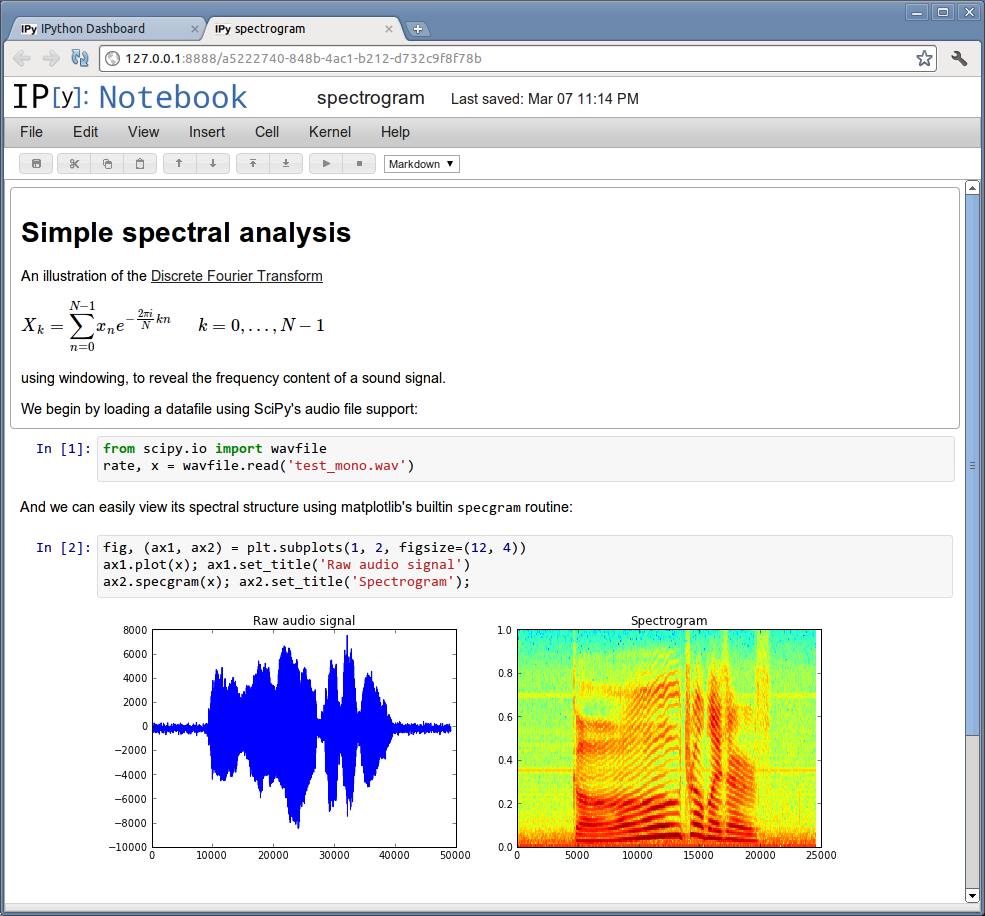
\includegraphics[width=3.2in]{fig/ipython-notebook-specgram.png}
\par\end{centering}

\caption{\label{fig:IPython-notebook}The web-based IPython Notebook combines
explanatory text, mathematics, multimedia, code and the results from
executing the code.}
\end{figure}



\section{Conclusion}\label{conclusion}

This is a large and complex problem that requires changing the educational
process for new scientists, the incentive models for promotions and
rewards, the publication system, and more.


\subsection{Changing culture}

Open{*}: software, access (Elsevier), education, review.

Internet: interactions for humans, code and data

\begin{itemize}
\item Open Source Software

\begin{itemize}
\item development akin to scientific culture
\item viable alternatives to proprietary software
\item tools and lessons for improving the scientific process: Github
\end{itemize}

\item Open Access

\begin{itemize}
\item \url{thecostofknowledge.org}: Elsevier boycott
\item FRPAA House hearing on March 29th.
\end{itemize}

\item Open Education

\begin{itemize}
\item MIT Open Courseware, Khan Academy\ldots
\item Stanford CS 221 in fall 2011: \textasciitilde{}160,000 students.
\item Spring 2012:

\begin{itemize}
\item Sebastian Thrun leaves Stanford: Udacity.
\item Stanford: Coursera.
\end{itemize}
\item MITx, TED-Ed\ldots
\end{itemize}
\end{itemize}

\subsection{Incentive models}

Science has become computational, but the incentive models of science
are single-mindedly focused on paper-oriented publications that completely
ignore the very existence of a computational process. Papers are accepted 

What role should journals play?

\begin{itemize}
\item Journals should mandate that upon paper \emph{approval} (but before
actual publication and with said publication being conditioned on
the author meeting this last condition), authors must expose their
version control system to the public, and that the publicly available
version can faithfully reproduce (within the limitations discussed
above) the published results. This public version then becomes available
for the scientific community not only for download, but also as a
starting point for further contribution and development.

\item supplemental material

\item peer review

\item new BioMed Central journal, Open Research Computation

 \item ongoing thematic series in Source Code for Biology and Medicine.
\cite{neylon2012changing}

\end{itemize}

How will all this impact scientists?

\begin{itemize}

\item funding
\item academic merit review

\end{itemize}

\subsection{Education and training}

\paragraph{ {\bf Workshops}}

\begin{itemize}

\item Software carpentry

\ldots basic training

\item Python

\ldots use of git

\end{itemize}

\paragraph{ {\bf Courses}}

\begin{itemize}

\item Josh

\item Randy

\item Titus

\end{itemize}


\section*{Acknowledgements}
We would like to thank
\begin{itemize}
\item members of the scientific Python community
\item scientist from various labs
\item Brian Granger
\item John Hunter
\item reviewers
\end{itemize}

\bibliographystyle{plain}
\bibliography{ipython}

\end{document}
